% =====================================================================
%  Proyecto Aprendizaje por Refuerzo - Cuarto 8x8 con obstáculos móviles
%  Entrega final: implementación, entrenamiento y evaluación
%  Compilar con pdfLaTeX:  latexmk -pdf reporte_final.tex
%  Las cifras de generado/ las produce experiments/cuarto_8x8/report_numbers.py
% =====================================================================
\documentclass[11pt,letterpaper]{article}

\usepackage[T1]{fontenc}
\usepackage[utf8]{inputenc}
\usepackage{babel}
\babelprovide[import,main]{spanish}
\usepackage{lmodern}
\usepackage[margin=2.3cm]{geometry}
\usepackage{fancyhdr}
\usepackage{titlesec}
\usepackage{parskip}
\usepackage{amsmath,amssymb}
\usepackage{booktabs}
\usepackage{tabularx}
\usepackage{array}
\usepackage[table]{xcolor}
\usepackage{enumitem}
\usepackage{caption}
\usepackage{graphicx}
\usepackage{float}
\usepackage{pdfpages}
\usepackage[colorlinks=true,linkcolor=azul,urlcolor=azul]{hyperref}

\definecolor{azul}{HTML}{1F4E79}
\titleformat{\section}{\Large\bfseries\color{azul}}{\thesection.}{0.6em}{}
\titleformat{\subsection}{\large\bfseries\color{azul}}{\thesubsection}{0.6em}{}
\captionsetup{font=small,labelfont=bf}
\setlist{itemsep=2pt,topsep=4pt}
\newcolumntype{L}{>{\raggedright\arraybackslash}X}
\newcolumntype{R}{>{\raggedleft\arraybackslash}X}
\newcolumntype{P}[1]{>{\raggedright\arraybackslash}p{#1}}
\renewcommand{\arraystretch}{1.25}
\setlength{\emergencystretch}{2em}
\graphicspath{{figuras/}{../../results/cuarto_8x8/figures/}{../../results/cuarto_8x8/grid/figures/}}

\pagestyle{fancy}
\fancyhf{}
\lhead{\small Aprendizaje por Refuerzo -- Proyecto, entrega final}
\rhead{\small Cuarto 8x8 con obstáculos móviles}
\cfoot{\small \thepage}

\newcommand{\IZQ}{\mathsf{GIRAR\_IZQ}}
\newcommand{\DER}{\mathsf{GIRAR\_DER}}
\newcommand{\AV}{\mathsf{AVANZAR}}
\newcommand{\META}{s_{\mathrm{META}}}
\newcommand{\COL}{s_{\mathrm{COL}}}
% Rutas en monoespaciada que pueden partirse después de / y _
\newcommand{\code}[1]{{\ttfamily\codebreaks#1\endcodebreaks}}
\makeatletter
\def\codebreaks#1\endcodebreaks{\@codebreaks#1\@nil}
\def\@codebreaks#1{\ifx#1\@nil\else\ifx#1/\slash\else\ifx#1\_\_\allowbreak\else#1\fi\fi\expandafter\@codebreaks\fi}
\makeatother
\makeatletter\newcommand{\filas}[1]{\@@input #1 }\makeatother

\newcommand{\QLExito}{35{,}1}
\newcommand{\QLExitoci}{2{,}1}
\newcommand{\QLChoque}{64{,}9}
\newcommand{\QLPasos}{16{,}0}
\newcommand{\QLCkpt}{30\,000}
\newcommand{\QLEstados}{252}
\newcommand{\SARSAExito}{34{,}4}
\newcommand{\SARSAExitoci}{2{,}1}
\newcommand{\SARSAChoque}{65{,}6}
\newcommand{\SARSAPasos}{17{,}0}
\newcommand{\SARSACkpt}{15\,000}
\newcommand{\SARSAEstados}{252}
\newcommand{\RandExito}{0{,}4}
\newcommand{\RandExitoci}{0{,}3}
\newcommand{\RandChoque}{99{,}6}
\newcommand{\RandPasos}{71{,}4}
\newcommand{\BordeExito}{35{,}1}
\newcommand{\BordeExitoci}{2{,}1}
\newcommand{\BordeChoque}{64{,}9}
\newcommand{\BordePasos}{16{,}0}
\newcommand{\EscExito}{15{,}9}
\newcommand{\EscExitoci}{1{,}6}
\newcommand{\EscChoque}{84{,}1}
\newcommand{\EscPasos}{28{,}0}
\newcommand{\SQLExito}{65{,}2}
\newcommand{\SQLExitoci}{2{,}1}
\newcommand{\SQLChoque}{34{,}8}
\newcommand{\SQLPasos}{23{,}5}
\newcommand{\SQLCkpt}{180\,000}
\newcommand{\SQLEstados}{3\,910}
\newcommand{\SSARSAExito}{62{,}9}
\newcommand{\SSARSAExitoci}{2{,}1}
\newcommand{\SSARSAChoque}{37{,}1}
\newcommand{\SSARSAPasos}{21{,}7}
\newcommand{\SSARSACkpt}{200\,000}
\newcommand{\SSARSAEstados}{3\,909}
\newcommand{\SRandExito}{0{,}4}
\newcommand{\SRandExitoci}{0{,}3}
\newcommand{\SRandChoque}{99{,}6}
\newcommand{\SRandPasos}{71{,}4}
\newcommand{\SBordeExito}{35{,}1}
\newcommand{\SBordeExitoci}{2{,}1}
\newcommand{\SBordeChoque}{64{,}9}
\newcommand{\SBordePasos}{16{,}0}
\newcommand{\SEscExito}{15{,}9}
\newcommand{\SEscExitoci}{1{,}6}
\newcommand{\SEscChoque}{84{,}1}
\newcommand{\SEscPasos}{28{,}0}
\newcommand{\SCautExito}{44{,}5}
\newcommand{\SCautExitoci}{2{,}2}
\newcommand{\SCautChoque}{55{,}5}
\newcommand{\SCautPasos}{22{,}3}
\newcommand{\Episodios}{50\,000}
\newcommand{\SEpisodios}{200\,000}
\newcommand{\TurnosPrueba}{2\,000}
\newcommand{\TurnosValidacion}{500}
\newcommand{\GammaF}{0{,}99}
\newcommand{\AlphaPot}{0{,}7}
\newcommand{\AlphaMin}{0{,}01}
\newcommand{\EpsIni}{1{,}0}
\newcommand{\EpsMin}{0{,}05}
\newcommand{\IgualBorde}{2\,000}
\newcommand{\DifQLEsc}{19{,}2}
\newcommand{\DifQLEscci}{2{,}6}
\newcommand{\DifQLRand}{34{,}7}
\newcommand{\DifQLRandci}{2{,}1}
\newcommand{\DifSensores}{30{,}1}
\newcommand{\DifSensoresci}{2{,}6}
\newcommand{\RutaQL}{DAAAAAAADAAAAAAA}
\newcommand{\RutaSARSA}{IIAAAAAAAIAAAAAAA}
\newcommand{\GirosQL}{2}
\newcommand{\GirosSARSA}{3}
\newcommand{\CausaAvanzando}{74}
\newcommand{\CausaCruce}{23}
\newcommand{\CausaGirando}{3}
\newcommand{\LugarFila}{63}
\newcommand{\LugarEsquina}{8}
\newcommand{\LugarColumna}{28}


\begin{document}

\begin{center}
  {\small Universidad de los Andes \textperiodcentered{} Maestría en Inteligencia Artificial}\\[2pt]
  {\small Aprendizaje por Refuerzo \textperiodcentered{} Prof. Nicolás Cardozo}\\[10pt]
  {\LARGE\bfseries\color{azul} Agente de RL en un cuarto 8x8\\[2pt] con obstáculos móviles}\\[8pt]
  {\large Entrega final: implementación, entrenamiento y evaluación}\\[8pt]
  Miguel Ángel Muñoz Layton \quad\textperiodcentered\quad Daniel F. Barrera Armendaris\\[2pt]
  {\small Noviembre de 2026}
\end{center}

\vspace{4pt}
\hrule
\vspace{8pt}

\section*{Resumen}

Se implementó el ambiente del enunciado con las reglas que aclaró el curso: un cuarto de $8\times8$ donde el
agente parte de $(0,0)$, debe llegar a $(7,7)$ y no puede chocar con cinco obstáculos que se mueven al azar al
mismo tiempo que él. El agente no ve los obstáculos, así que su Q-tabla depende solo de su posición y su
orientación. Se entrenaron agentes de Q-learning y SARSA durante \Episodios{} episodios, con hiperparámetros
elegidos en una búsqueda en grid de \GridTotal{} combinaciones evaluadas solo en validación. Sin entrenar, el
agente llega a la meta en el \RandExito\,\% de los episodios. Entrenado con Q-learning llega en el
\textbf{\QLExito\,\%}, y lo hace por una ruta que nadie le indicó: va por el borde del cuarto, primero hacia
abajo por la columna 0 y luego hacia la derecha por la fila 7. Es estadísticamente igual a la mejor regla que
diseñamos a mano (la ruta espejo, por la fila 0 y la columna 7) y supera en \DifQLEsc{} $\pm$ \DifQLEscci{} puntos
a la ruta en escalera por el centro. La búsqueda de hiperparámetros muestra que con $\gamma\le0{,}95$ el agente se
queda girando en la salida y que con $\gamma\ge0{,}99$ todas las combinaciones aprenden una ruta por el borde. La
Q-tabla se guarda y se carga desde un archivo, y el video muestra al agente usando esa Q-tabla.

% =====================================================================
\section{Definición del problema}

\subsection{Cambios desde la Entrega 1}

En la Entrega 1 definimos por error otro problema (la consolidación de pedidos en una bodega), no el del
enunciado. Para esta entrega rehicimos la definición completa sobre el ambiente del curso, el cuarto de
$8\times8$ con cinco obstáculos móviles, siguiendo las aclaraciones del foro y de los monitores. Cambiaron los
tres componentes:
\begin{itemize}
  \item \textbf{Estados:} posición y orientación del agente, posiciones de los cinco obstáculos, inicio en
    $(0,0)$, meta en $(7,7)$ y los terminales de llegada ($\META$) y de colisión ($\COL$).
  \item \textbf{Acciones:} girar $90^\circ$ a la izquierda, girar $90^\circ$ a la derecha y avanzar a la casilla
    de enfrente si existe, con el conjunto de acciones disponibles $A(s)$ en cada casilla del tablero.
  \item \textbf{Recompensas:} $+100$ al llegar a $(7,7)$, $-100$ al chocar con un obstáculo y $-1$ por cada paso
    y cada giro.
\end{itemize}
La definición completa, con la definición formal de los terminales y diez triplas $(s,a,s')$ verificadas con
pruebas automáticas, está en el \hyperref[anexo]{Anexo A}. El cuadro~\ref{tab:mdp} la resume.

\subsection{Resumen del MDP}

\begin{table}[H]
\centering\small
\begin{tabularx}{\textwidth}{@{}P{2.4cm}L@{}}
\toprule
\textbf{Elemento} & \textbf{Definición} \\
\midrule
Estado del ambiente & $s=(f,c,\theta,o_1,\dots,o_5)$: posición y orientación del agente ($\theta\in\{\mathrm{N,E,S,O}\}$) y posiciones de los cinco obstáculos. Inicio: $(0,0)$ mirando al norte, obstáculos al azar. Terminales: $\META$ (llega a $(7,7)$) y $\COL$ (choca); en ambos el episodio termina y el ambiente se reinicia en $(0,0)$ con obstáculos nuevos. Sin límite de pasos \\
Observación del agente & $(f,c,\theta)$: el agente es ciego, sin sensores; no ve los obstáculos y solo se entera chocando. Es la clave de la Q-tabla: 256 filas por 3 acciones \\
Acciones & $\IZQ$ y $\DER$ (girar $90^\circ$; siempre aplicables) y $\AV$ (a la casilla de enfrente; solo si existe) \\
Dinámica & Aleatoria: cada obstáculo se queda o pasa a una vecina al azar, con igual probabilidad (nunca a la salida ni a la meta, ni encima de otro), al mismo tiempo que el agente. Hay colisión si comparten casilla o se cruzan, también mientras el agente gira \\
Recompensa & $+100$ al llegar a $(7,7)$; $-100$ al chocar; $-1$ por cada paso y cada giro; $-10$ por avanzar contra la pared (no ocurre con la máscara $A(s)$). $\gamma=\GammaF$ \\
\bottomrule
\end{tabularx}
\caption{Resumen del MDP.}
\label{tab:mdp}
\end{table}

% =====================================================================
\section{Implementación}

El código está en el repositorio \href{https://github.com/panamiguell/rl-warehouse-agent}{panamiguell/rl-warehouse-agent}:

\begin{itemize}
  \item \code{src/rl\_gridworld/env.py}: el ambiente, compatible con Gymnasium. \code{reset} ubica al agente y
    los obstáculos; \code{step} aplica la acción, mueve los obstáculos, detecta colisiones y devuelve la
    recompensa; \code{action\_mask} da $A(s)$; \code{observe} entrega $(f,c,\theta)$.
  \item \code{src/rl\_gridworld/agent.py}: los agentes tabulares (Q-learning y SARSA) y la memoria del agente.
    \code{TabularAgent.save(ruta)} guarda la Q-tabla con sus hiperparámetros en un archivo \code{.npz}, y
    \code{TabularAgent.load(ruta)} la carga en un agente listo para actuar. La Q-tabla también se exporta
    legible en CSV: una fila por estado y una columna por acción.
  \item \code{src/rl\_gridworld/baselines.py}: reglas fijas de referencia que, como el agente, no ven los
    obstáculos. La \emph{aleatoria} hace lo mismo que el agente antes de entrenar. La regla \emph{por el borde}
    va hacia la derecha por la fila 0 y luego hacia abajo por la columna 7. La regla \emph{escalera} alterna
    derecha y abajo por la diagonal. Las dos últimas son caminos de longitud mínima (14 avances).
  \item \code{experiments/cuarto\_8x8/}: entrenamiento y evaluación (\code{train.py}), video (\code{demo.py})
    y cifras de este reporte (\code{report\_numbers.py}).
  \item \code{tests/test\_gridworld.py}: 18 pruebas automáticas, entre ellas cada tripla $(s,a,s')$ del
    documento de definición, que el agente no ve los obstáculos y el guardar/cargar de la Q-tabla.
\end{itemize}

\textbf{Actualizaciones.} Con $\delta = r + \gamma\,\hat{Q}(x') - Q(x,a)$ y $Q(x,a)\leftarrow Q(x,a)+\alpha_t\,\delta$,
Q-learning usa $\hat{Q}(x')=\max_{a'\in A(x')}Q(x',a')$ y SARSA usa $\hat{Q}(x')=Q(x',a')$ con la acción que
realmente toma (Sutton y Barto, 2018, secs.~6.4 y~6.5). En $\META$ y $\COL$, $\hat{Q}(x')=0$. Como el agente no ve los obstáculos, la misma acción en la
misma casilla a veces termina en choque y a veces no: las recompensas son muy ruidosas. Por eso probamos,
además de una $\alpha$ fija, una tasa que disminuye con las visitas a cada par,
$\alpha_t(x,a)=\max(0{,}01,\ N(x,a)^{-\omega})$. Los valores de $\gamma$, $\alpha$ y $\varepsilon$ se eligieron
con la búsqueda de la sección~\ref{sec:grid}; el cuadro~\ref{tab:hiper} muestra los elegidos.

\begin{table}[H]
\centering\small
\begin{tabularx}{\textwidth}{@{}P{5.4cm}L@{}}
\toprule
\textbf{Parámetro} & \textbf{Valor} \\
\midrule
Episodios de entrenamiento & \Episodios{} por algoritmo \\
Tasa de aprendizaje & $\alpha_t(x,a)=\max(\AlphaMin,\ N(x,a)^{-\AlphaPot})$ \\
Descuento $\gamma$ & \GammaF{} \\
Exploración $\varepsilon$ & De \EpsIni{} a \EpsMin{}, decaimiento geométrico hasta el 80\,\% del entrenamiento \\
Inicialización de la Q-tabla & $Q=0$ \\
Evaluación & Política greedy (sin exploración) \\
Semillas & Entrenamiento, validación y prueba disjuntas \\
Q-tabla entregada & La del mejor punto de control en validación (\TurnosValidacion{} episodios cada 5\,000): episodio \QLCkpt{} \\
Evaluación final & \TurnosPrueba{} episodios de prueba, los mismos para agentes y reglas \\
\bottomrule
\end{tabularx}
\caption{Hiperparámetros elegidos con la búsqueda de la sección~\ref{sec:grid} y protocolo.}
\label{tab:hiper}
\end{table}

% =====================================================================
\section{Búsqueda de hiperparámetros}
\label{sec:grid}

Exploramos un grid de hiperparámetros con \code{experiments/cuarto\_8x8/grid\_search.py}: \GridTotal{}
combinaciones, cada una entrenada \Episodios{} episodios, más \GridConfirmacion{} corridas de confirmación con
otras semillas. Para no elegir con los datos con los que se reporta, la búsqueda usa solo episodios de
\emph{validación}; los de prueba se usan una sola vez, con la configuración elegida. Para cada combinación se
guarda el mejor punto de control (500 episodios de validación cada 5\,000 de entrenamiento) y se vuelve a evaluar
en 2\,000 episodios de validación nuevos, para no elegir por la suerte de los primeros 500.

\textbf{Hipótesis.} Antes de correr la búsqueda escribimos qué esperábamos (están en el código del script):
\begin{itemize}
  \item \textbf{H1, $\gamma$ bajo.} Con $\gamma=0{,}90$ o $0{,}95$ el agente se queda girando en la salida, que es
    segura: girar sin fin vale $-1/(1-\gamma)=-10$ o $-20$, más que intentar llegar con cerca de 65\,\% de
    choques. Esta hipótesis venía de una primera versión con $\gamma=0{,}95$ en la que vimos ese comportamiento.
  \item \textbf{H2, $\gamma$ alto.} Con $\gamma=0{,}999$ también sale (girar sin fin vale $-1\,000$), pero como los
    valores son más grandes y ruidosos, aprende igual o un poco peor que con $0{,}99$.
  \item \textbf{H3, tasa de aprendizaje.} Con $\alpha$ fija los valores oscilan por el ruido de los choques y la
    política es menos estable; la tasa por visitas converge mejor.
  \item \textbf{H4, exploración.} El $\varepsilon$ mínimo casi no cambia la ruta final, porque se evalúa la política
    greedy.
  \item \textbf{H5, algoritmo.} Q-learning y SARSA llegan a resultados parecidos: sin ver los obstáculos, lo único
    que se puede aprender es la ruta.
\end{itemize}

\subsection{Etapa 1: el descuento \texorpdfstring{$\gamma$}{gamma}}

Probamos $\gamma\in\{0{,}90;\ 0{,}95;\ 0{,}99\}$ con los dos algoritmos ($\omega=0{,}7$ y $\varepsilon$ mínimo
$0{,}05$). Con $\gamma$ bajo el agente gira en la salida hasta el corte de seguridad, así que en esta etapa el
corte de entrenamiento se bajó a 200 pasos para que el cómputo cupiera. No cambia lo que se aprende: en el corte
no se trata el estado como terminal y se sigue estimando su valor.

\begin{table}[H]
\centering\small
\begin{tabularx}{\textwidth}{@{}lcrLr@{}}
\toprule
\textbf{Algoritmo} & $\boldsymbol{\gamma}$ & \textbf{Llega (\%)} & \textbf{Qué aprende} & \textbf{Pasos por episodio} \\
\midrule
\filas{generado/tabla_gamma.tex}
\bottomrule
\end{tabularx}
\caption{Etapa 1. ``Llega'': episodios de validación que llegan a la meta con el mejor punto de control. ``Pasos
por episodio'': promedio durante el entrenamiento.}
\label{tab:gamma}
\end{table}

\subsection{Etapa 2: grid factorial}

Con $\gamma$ ya en la zona en que el agente sale, probamos todas las combinaciones de algoritmo (2), $\gamma\in\{0{,}99;\
0{,}999\}$ (2), tasa de aprendizaje (4: $\alpha$ fija $0{,}1$, o por visitas con $\omega\in\{0{,}5;\ 0{,}7;\
0{,}9\}$) y $\varepsilon$ mínimo $\in\{0{,}01;\ 0{,}05;\ 0{,}10\}$ (3): \GridEtapaDos{} combinaciones con el
ambiente oficial.

\begin{figure}[H]
\centering
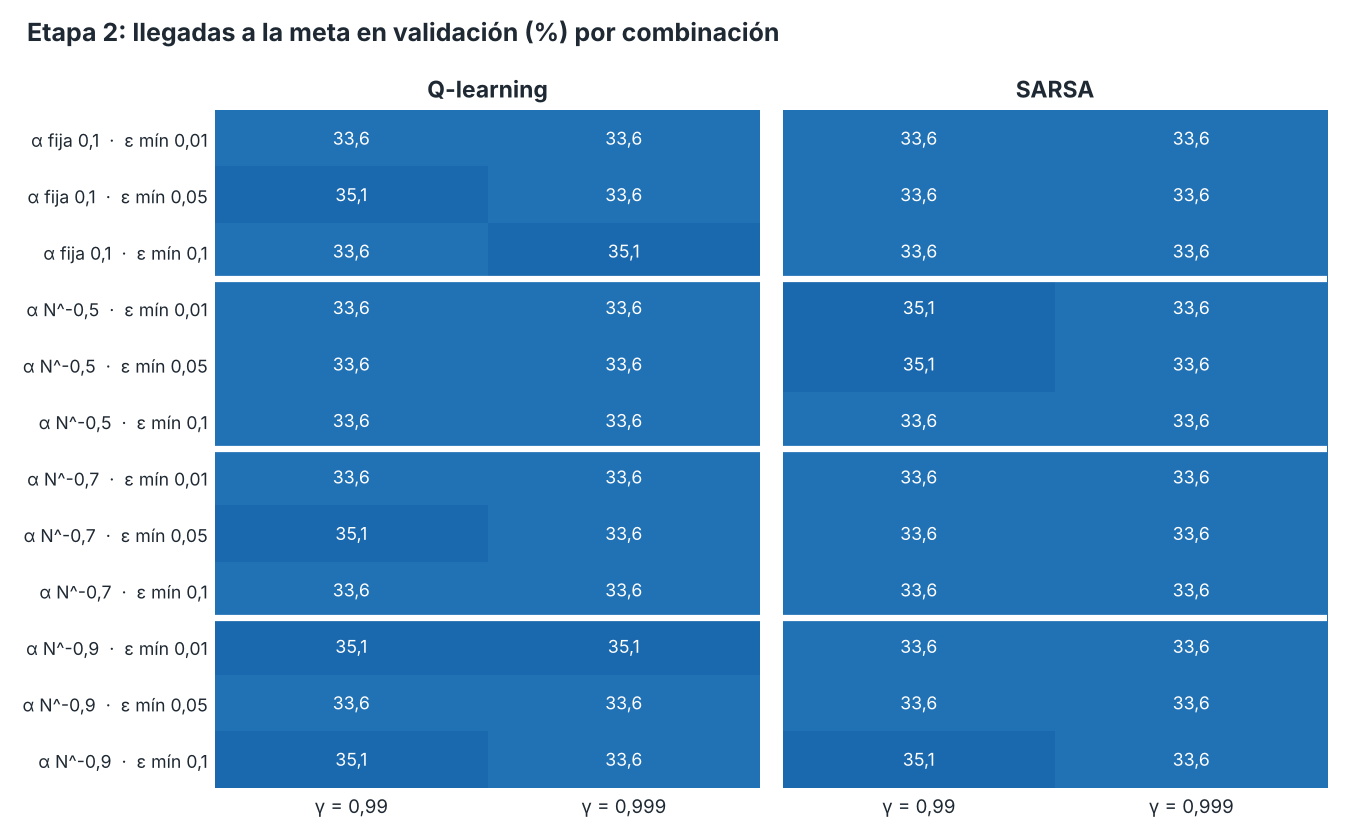
\includegraphics[width=0.86\textwidth]{grid.png}
\caption{Etapa 2: porcentaje de episodios de validación que llegan a la meta en cada combinación.}
\label{fig:grid}
\end{figure}

Las \GridBorde{} de las \GridEtapaDos{} combinaciones aprenden una ruta por el borde, y las llegadas en validación
solo van de \GridMin\,\% a \GridMax\,\%. Esa diferencia no viene de los hiperparámetros sino de cuál de las dos
rutas por el borde aprende cada corrida: \GridFilaCero{} aprendieron la de la fila 0 y la columna 7
(\GridValFilaCero\,\% en validación) y \GridColumnaCero{} la de la columna 0 y la fila 7 (\GridValColumnaCero\,\%).
Con 2\,000 episodios, una diferencia así está dentro del intervalo de confianza ($\pm$2 puntos). Donde sí se nota
la tasa de aprendizaje es en la estabilidad: con $\alpha$ fija, en promedio \GridCerosFija{} de los 10 puntos de
control quedan en 0\,\% de llegadas y el mejor punto llega hacia el episodio \GridEpisodioFija{}; con la tasa por
visitas, \GridCerosVisitas{} puntos en 0\,\% y el mejor hacia el episodio \GridEpisodioVisitas{}. El promedio de
llegadas en validación es casi el mismo para Q-learning (\GridValQL\,\%) y SARSA (\GridValSARSA\,\%), para
$\gamma=0{,}99$ (\GridValGammaNN\,\%) y $0{,}999$ (\GridValGammaNNN\,\%), y para los tres $\varepsilon$ mínimos
(\GridValEpsUno\,\%, \GridValEpsCinco\,\% y \GridValEpsDiez\,\%).

\subsection{Confirmación con otras semillas y elección}

Las cinco mejores combinaciones de la etapa 2 se repitieron con dos semillas de entrenamiento más. Gana la de
mayor promedio en validación.

\begin{table}[H]
\centering\small
\begin{tabularx}{\textwidth}{@{}lcccrrrrL@{}}
\toprule
\textbf{Algoritmo} & $\boldsymbol{\gamma}$ & $\boldsymbol{\alpha}$ & $\boldsymbol{\varepsilon}$ \textbf{mín} & \textbf{Sem. 0} & \textbf{Sem. 1} & \textbf{Sem. 2} & \textbf{Prom.} & \textbf{Ruta aprendida} \\
\midrule
\filas{generado/tabla_confirmacion.tex}
\bottomrule
\end{tabularx}
\caption{Confirmación: llegadas en validación (\%) con tres semillas de entrenamiento.}
\label{tab:confirmacion}
\end{table}

La configuración elegida es \textbf{\SelAlg{} con $\gamma=\SelGamma$, tasa por visitas con $\omega=\SelOmega$ y
$\varepsilon$ mínimo \SelEps} (\SelVal\,\% en validación). Empata en promedio con la misma configuración con
$\gamma=0{,}99$; el desempate por estabilidad eligió $0{,}999$. La conclusión importante del grid es otra: dentro de
la zona en que el agente sale de la salida, los hiperparámetros casi no cambian el resultado. La misma
configuración aprende una u otra ruta según la semilla, y las dos rutas llegan a la meta en proporciones que no
se pueden distinguir con los datos. Con este agente ciego, lo que se puede aprender es la ruta, y todas las
configuraciones razonables encuentran una ruta por el borde.

% =====================================================================
\section{Resultados}

\subsection{Curvas de aprendizaje}

\begin{figure}[H]
\centering
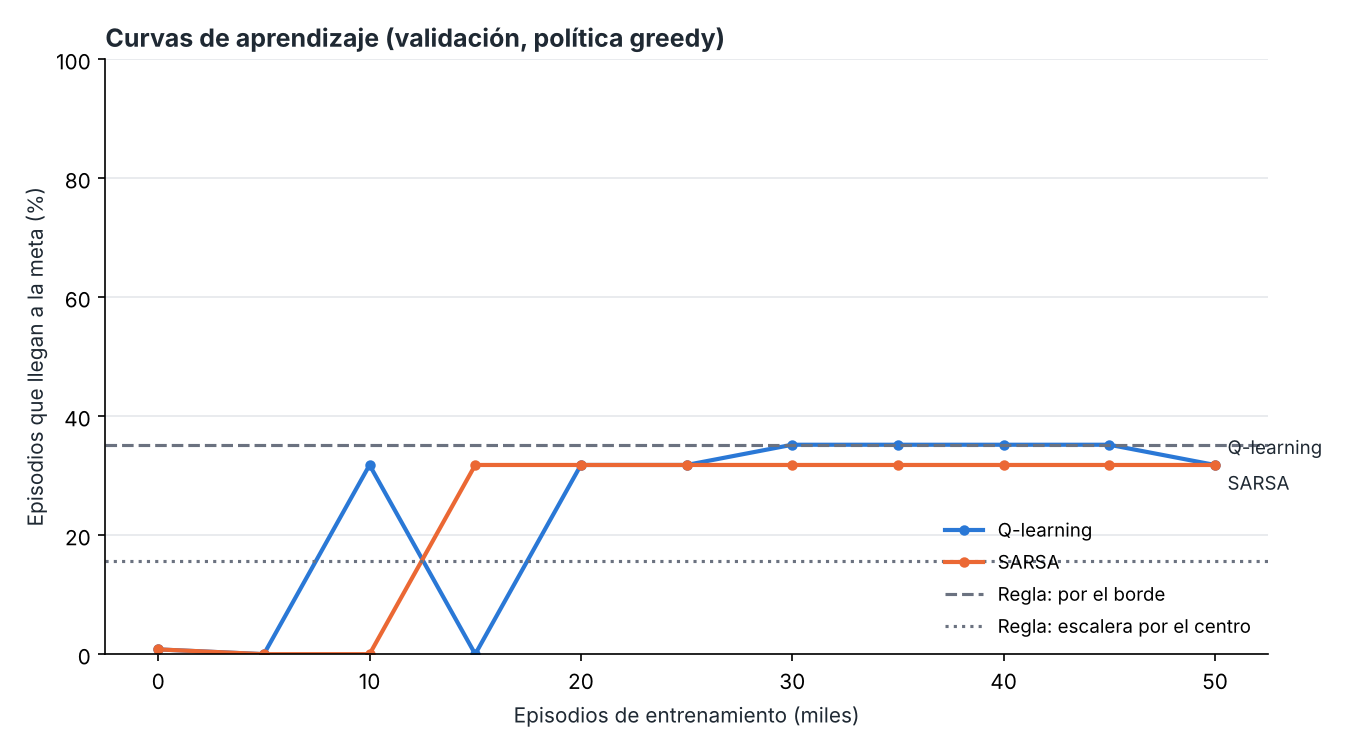
\includegraphics[width=0.78\textwidth]{curvas_aprendizaje.png}
\caption{Porcentaje de episodios de validación que llegan a la meta durante el entrenamiento.}
\label{fig:curvas}
\end{figure}

Antes de entrenar, la Q-tabla está en ceros y el agente actúa al azar: casi nunca llega a la meta. En los
primeros puntos de control, mientras explora mucho, la política greedy todavía queda girando en un mismo sitio
(0\,\% de llegadas). Q-learning fija su ruta a los \QLCkpt{} episodios y SARSA a los \SARSACkpt{}; desde ahí la
política greedy ya no cambia. Las dos curvas quedan a la altura de la regla por el borde: Q-learning con la ruta
espejo de esa regla y SARSA con la misma ruta de la regla.

\subsection{Evaluación en prueba}

\begin{table}[H]
\centering\small
\begin{tabularx}{\textwidth}{@{}Lrrrrr@{}}
\toprule
\textbf{Política} & \textbf{Llega (\%)} & \textbf{Choca (\%)} & \textbf{Sin terminar (\%)} & \textbf{Pasos si llega} & \textbf{Recompensa} \\
\midrule
\filas{generado/tabla_resultados.tex}
\bottomrule
\end{tabularx}
\caption{Resultados en \TurnosPrueba{} episodios de prueba ($\pm$: intervalo de confianza del 95\,\%).
``Sin terminar'' son los episodios que llegarían al corte de seguridad de 1\,000 pasos.}
\label{tab:resultados}
\end{table}

\begin{figure}[H]
\centering
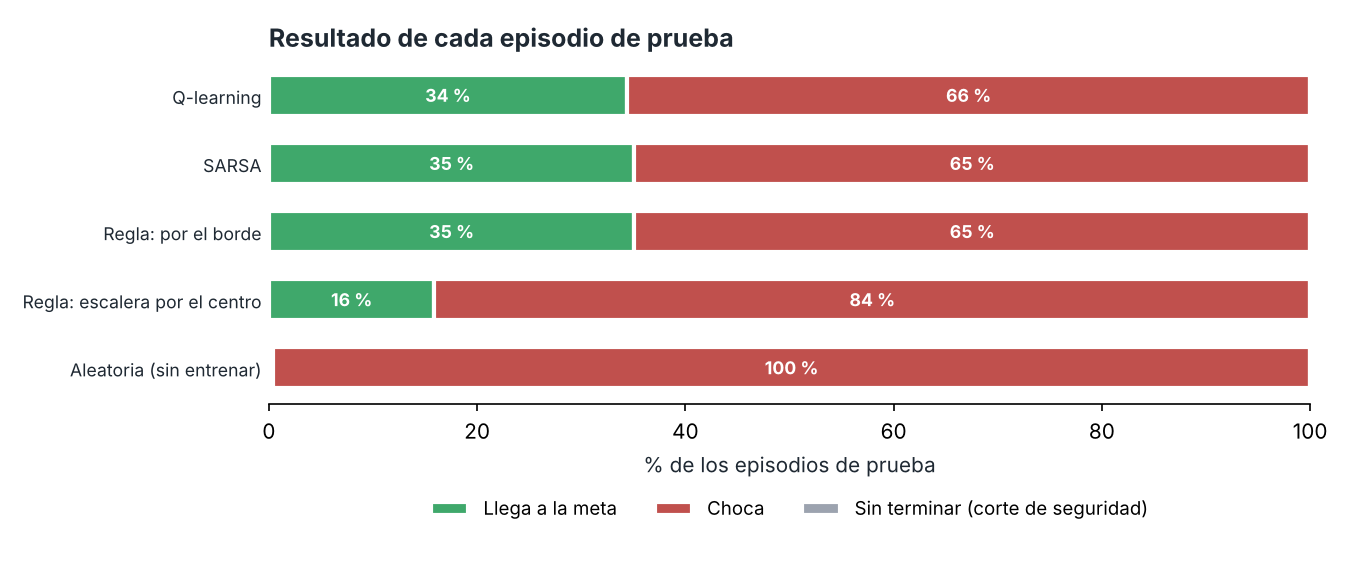
\includegraphics[width=0.78\textwidth]{comparacion.png}
\caption{Cómo termina cada episodio de prueba.}
\end{figure}

Todas las políticas se evaluaron en los mismos episodios: misma posición inicial y mismos movimientos
aleatorios de los obstáculos, así que las diferencias se miden episodio a episodio. Frente al agente sin
entrenar, Q-learning llega a la meta en \DifQLRand{} $\pm$ \DifQLRandci{} puntos porcentuales más de episodios, y
supera a la escalera por el centro en \DifQLEsc{} $\pm$ \DifQLEscci{} puntos. Frente a la regla por el borde la
diferencia es de \DifQLBorde{} $\pm$ \DifQLBordeci{} puntos: no se distingue de cero. Q-learning toma la ruta
espejo de esa regla y SARSA exactamente la misma, así que SARSA y la regla tienen el mismo resultado. Ningún
episodio quedó sin terminar: el agente siempre avanza hacia la meta.

\subsection{Qué aprendió el agente: la ruta}
\label{sec:ruta}

Como el agente no ve los obstáculos, su política depende solo de dónde está y hacia dónde mira, así que es una
ruta fija. La figura~\ref{fig:ruta} la muestra.

\begin{figure}[H]
\centering
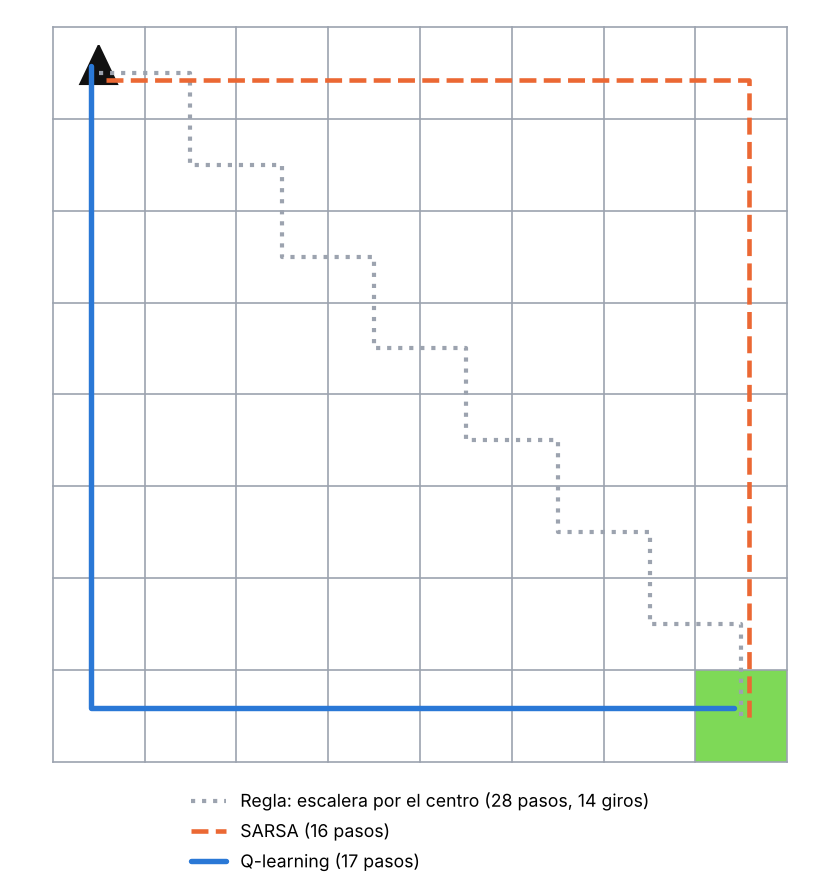
\includegraphics[width=0.46\textwidth]{ruta_aprendida.png}
\caption{Rutas de la política greedy aprendida y de la regla en escalera.}
\label{fig:ruta}
\end{figure}

Q-learning aprendió la secuencia \code{\RutaQL} (D: girar a la derecha, I: girar a la izquierda, A: avanzar):
gira dos veces hasta mirar al sur, baja por la columna 0, gira hacia el este y recorre la fila 7. Son \PasosQL{}
pasos con \GirosQL{} giros. SARSA aprendió la ruta espejo (\code{\RutaSARSA}): gira hacia el este, recorre la
fila 0, gira hacia el sur y baja por la columna 7, con \PasosSARSA{} pasos y \GirosSARSA{} giros; es la misma
ruta de la regla por el borde. Como el agente empieza mirando al norte, la ruta por la columna 0 necesita un giro
más, y aun así las dos llegan en proporciones que no se distinguen. Que estas rutas sean mejores que la escalera,
con el mismo número de avances, tiene dos explicaciones:
\begin{itemize}
  \item \textbf{Menos giros.} Cada giro es un paso más en el que un obstáculo puede llegar. La escalera necesita
    14 giros y tarda 28 pasos; las rutas por el borde, 2 o 3 giros y 16 o 17 pasos.
  \item \textbf{Menos vecinas.} Una casilla del borde tiene 3 vecinas (2 en las esquinas) desde las que un
    obstáculo puede entrar; una casilla interior tiene 4.
\end{itemize}
De los choques de Q-learning, el \CausaAvanzando\,\% ocurre al avanzar hacia una casilla en la que entra o se
queda un obstáculo, el \CausaCruce\,\% al cruzarse con uno y el \CausaGirando\,\% mientras gira. El
\LugarUno\,\% ocurre en la \TramoUno, el \LugarEsquina\,\% en la esquina \Esquina{} y el \LugarDos\,\% en la
\TramoDos.

\subsection{La Q-tabla}
\label{sec:qtabla}

La Q-tabla de Q-learning tiene \QLEstados{} de los 252 estados no terminales: el agente los visitó todos
mientras exploraba. Se entrega completa en \code{results/cuarto\_8x8/models/q\_learning\_qtable.csv}. El
cuadro~\ref{tab:qtabla} muestra algunas filas; en negrita, la acción que elige el agente.

\begin{table}[H]
\centering\small
\begin{tabularx}{\textwidth}{@{}P{1.6cm}cRRR@{}}
\toprule
$(f,c)$ & $\theta$ & $Q(\IZQ)$ & $Q(\DER)$ & $Q(\AV)$ \\
\midrule
\filas{generado/tabla_qtabla.tex}
\bottomrule
\end{tabularx}
\caption{Extracto de la Q-tabla de Q-learning (n/a: acción no aplicable).}
\label{tab:qtabla}
\end{table}

Los valores reflejan la ruta. En $(0,0)$ mirando al norte solo se puede girar, y los dos giros valen casi lo
mismo, porque por cualquiera de los dos lados se llega a mirar al sur en dos giros. Mirando al sur, en la columna
0, lo mejor es avanzar. En la esquina $(7,0)$ mirando al sur, girar a la izquierda. En la fila 7 mirando al este,
avanzar, y en $(7,6)$ ese avance vale exactamente $+100$. Los valores crecen a lo largo de la ruta, de
\QSalida{} en la salida a $+100$ junto a la meta. En la salida son negativos porque el agente choca antes de
llegar en cerca de dos de cada tres episodios; el valor es cercano a la recompensa media por episodio del
cuadro~\ref{tab:resultados}. La última fila, $(3,3)$, es una casilla fuera de la ruta: el agente la visitó
mientras exploraba, pero nunca pasa por ella con la política greedy.

% =====================================================================
\section{Comportamiento esperado y comportamiento observado}
\label{sec:comportamiento}

Para cada experimento escribimos antes de correrlo qué creíamos que iba a pasar, y lo comparamos con lo que
ocurrió.

\begin{table}[H]
\centering\small
\begin{tabularx}{\textwidth}{@{}P{3.3cm}LL@{}}
\toprule
\textbf{Experimento y condiciones} & \textbf{Lo que esperábamos} & \textbf{Lo que ocurrió} \\
\midrule
H1. $\gamma=0{,}90$ y $0{,}95$ (cuadro~\ref{tab:gamma}) & Que el agente se quedara girando en la salida, porque
girar sin fin vale $-10$ o $-20$, más que intentar llegar & \textbf{Se cumplió.} Con los dos algoritmos llega en
el 0\,\% y su política greedy gira en $(0,0)$; durante el entrenamiento los episodios duran en promedio
\GammaPasosA{} pasos, contra \GammaPasosC{} con $\gamma=0{,}99$ \\
H2. $\gamma=0{,}999$ frente a $0{,}99$ (figura~\ref{fig:grid}) & Que también saliera, pero aprendiera igual o un
poco peor por tener valores más grandes y ruidosos & \textbf{Se cumplió en parte.} Sale y aprende una ruta por el
borde, pero no aprende peor: \GridValGammaNNN\,\% frente a \GridValGammaNN\,\% en validación, dentro del ruido \\
H3. $\alpha$ fija $0{,}1$ frente a tasa por visitas & Que con $\alpha$ fija la política fuera menos estable &
\textbf{Se cumplió.} Con $\alpha$ fija quedan en 0\,\% \GridCerosFija{} de 10 puntos de control y el mejor llega
hacia el episodio \GridEpisodioFija; con la tasa por visitas, \GridCerosVisitas{} y \GridEpisodioVisitas. Al final
las dos aprenden una ruta por el borde \\
H4. $\varepsilon$ mínimo $0{,}01$, $0{,}05$ y $0{,}10$ & Que casi no cambiara la ruta final & \textbf{Se
cumplió.} \GridValEpsUno\,\%, \GridValEpsCinco\,\% y \GridValEpsDiez\,\% en validación \\
H5. Q-learning frente a SARSA & Resultados parecidos, porque sin ver los obstáculos solo se puede aprender la
ruta & \textbf{Se cumplió.} \GridValQL\,\% y \GridValSARSA\,\% en el grid; \QLExito\,\% y \SARSAExito\,\% en
prueba \\
Agente final en prueba (sección~\ref{sec:ruta}) & Una ruta corta con pocos giros, sin avanzar nunca contra una
pared, y cerca de un tercio de llegadas, porque los choques dependen de obstáculos que no ve & \textbf{Se
cumplió.} Ruta por el borde de \PasosQL{} pasos y \GirosQL{} giros; llega en el \QLExito\,\%, choca en el
\QLChoque\,\% y ningún episodio queda sin terminar \\
Video (\VideoEpisodios{} episodios) & Cerca de un tercio de llegadas, como en prueba & Llegó en
\VideoMeta{} (\VideoExito\,\%): más de lo esperado, por el azar de una muestra pequeña
(sección~\ref{sec:entregables}) \\
\bottomrule
\end{tabularx}
\caption{Comportamiento esperado y observado en cada experimento.}
\label{tab:comportamiento}
\end{table}

\subsection{Comportamiento no esperado observado}

\begin{itemize}
  \item \textbf{El agente no salía de la salida.} En la primera versión usamos $\gamma=0{,}95$ sin pensar en este
    efecto, y el agente aprendió a quedarse girando para siempre en $(0,0)$. Como los obstáculos no entran en la
    salida y no hay límite de pasos, girar ahí no tiene riesgo, y con ese $\gamma$ vale más que intentar el
    recorrido con cerca de 65\,\% de choques. Era la política correcta para esas recompensas, pero no la que
    buscábamos. De ahí salió la hipótesis H1, que el grid confirmó para $\gamma=0{,}90$ y $0{,}95$ con los dos
    algoritmos.
  \item \textbf{La ruta depende de la semilla.} Esperábamos que cada configuración aprendiera siempre la misma
    ruta. En cambio, la misma configuración aprende a veces la ruta por la fila 0 y a veces la de la columna 0
    (cuadro~\ref{tab:confirmacion}). Las dos son igual de buenas, así que pequeñas diferencias en la exploración
    deciden cuál fija el agente. Por eso en el agente final Q-learning y SARSA terminaron con rutas espejo.
  \item \textbf{La política greedy gira en un mismo sitio al principio.} Mientras la Q-tabla tiene muchos
    valores sin aprender (en cero), la acción de mayor valor puede ser girar, y en los primeros puntos de control
    el agente greedy queda dando vueltas (0\,\% en la figura~\ref{fig:curvas}). Desaparece cuando el agente
    aprende los valores de la ruta. Por eso se entrega la Q-tabla del mejor punto de control en validación.
  \item \textbf{El video tuvo más llegadas que la prueba.} En los \VideoEpisodios{} episodios del video el agente
    llega \VideoMeta{} veces (\VideoExito\,\%), frente al \QLExito\,\% en prueba. No es un cambio de comportamiento:
    con \TurnosPrueba{} episodios a partir de las mismas semillas del video llega en el \VideoExitoLargo\,\%.
  \item \textbf{Choques mientras gira.} Las reglas lo permiten, pero no lo habíamos pensado como causa
    importante: es el \CausaGirando\,\% de los choques del agente final.
\end{itemize}

\subsection{Limitaciones}

\begin{itemize}
  \item Sin ver los obstáculos, ninguna política puede esquivarlos: lo único que se puede aprender es la ruta
    con menos riesgo esperado. Por eso el agente choca en cerca de dos de cada tres episodios.
  \item El agente iguala a la mejor regla fija, pero no la supera: con la información disponible, la ruta por el
    borde parece ser la mejor posible. No lo demostramos formalmente.
\end{itemize}

% =====================================================================
\section{Tiempo de ejecución y condiciones de hardware y software}

La búsqueda de hiperparámetros se corrió con \code{grid\_search.py} y el entrenamiento y la evaluación finales con \code{experiments/cuarto\_8x8/train.py}, que registra los
tiempos y el equipo en \code{results/cuarto\_8x8/logs/summary.json}. El código es Python de un solo hilo: usa
un núcleo del procesador y no usa GPU. El cuadro~\ref{tab:tiempos} resume el equipo, el software y los tiempos.

\begin{table}[H]
\centering\small
\begin{tabularx}{\textwidth}{@{}P{4.3cm}L@{}}
\toprule
\textbf{Elemento} & \textbf{Valor} \\
\midrule
Equipo & \CPU{} (\Nucleos{} núcleos virtuales), \RAM{} GB de RAM, sin GPU \\
Sistema operativo & \SO{} (máquina virtual en la nube) \\
Software & Python \VerPy{}, NumPy \VerNumpy{}, Gymnasium \VerGym{}, Matplotlib \VerMpl{}, PyYAML \VerYaml{} \\
\midrule
Entrenar Q-learning & \TQLEnt{} por \Episodios{} episodios (\TQLMsEp{} ms cada uno); \TQLEntVal{} con validaciones \\
Entrenar SARSA & \TSARSAEnt{} por \Episodios{} episodios (\TSARSAMsEp{} ms cada uno); \TSARSAEntVal{} con validaciones \\
Prueba & \TQLPrueba{} por agente (\TurnosPrueba{} episodios) \\
Corrida completa de \code{train.py} & \TTotal{} (dos agentes, cinco políticas evaluadas y figuras) \\
Búsqueda de hiperparámetros & \GridMinutos{} min (\GridTotal{} combinaciones y \GridConfirmacion{} corridas de confirmación, dos en paralelo) \\
Generar el video & \TVideo{} (\VideoEpisodios{} episodios) \\
\bottomrule
\end{tabularx}
\caption{Equipo, software y tiempos de ejecución.}
\label{tab:tiempos}
\end{table}

El entrenamiento es rápido porque la Q-tabla es pequeña: \QLEstados{} estados por 3 acciones, y cada episodio
dura pocos pasos. La corrida es determinista: con las mismas semillas,
volver a entrenar reproduce exactamente la misma Q-tabla y los mismos resultados.

% =====================================================================
\section{Entregables y reproducción}
\label{sec:entregables}

\begin{table}[H]
\centering\small
\begin{tabularx}{\textwidth}{@{}P{7.6cm}L@{}}
\toprule
\textbf{Archivo} & \textbf{Contenido} \\
\midrule
\code{results/cuarto\_8x8/figures/demo.mp4} & Video: \VideoEpisodios{} episodios del agente (\VideoDuracion{} min) con la Q-tabla cargada desde el archivo \\
\code{results/cuarto\_8x8/models/q\_learning.npz} & Q-tabla del agente (se carga con \code{TabularAgent.load}) \\
\code{results/cuarto\_8x8/models/*\_qtable.csv} & Q-tablas legibles de Q-learning y SARSA \\
\code{results/cuarto\_8x8/logs/} & Registros de las pruebas: entrenamiento, curvas, cada episodio de prueba y resúmenes \\
\code{src/rl\_gridworld/}, \code{experiments/cuarto\_8x8/}, \code{tests/} & Código completo \\
\bottomrule
\end{tabularx}
\caption{Entregables.}
\end{table}

\textbf{El video.} Muestra \VideoEpisodios{} episodios seguidos, con semillas que no se usaron ni al entrenar ni
al evaluar, y el agente actuando siempre con la acción de mayor valor en la Q-tabla cargada. Llega a la meta en
\VideoMeta{} de los \VideoEpisodios{} (\VideoExito\,\%) y choca en los demás. Es distinto del \QLExito\,\% de la
prueba porque \VideoEpisodios{} episodios son una muestra pequeña: con \TurnosPrueba{} episodios a partir de las
mismas semillas del video, el agente llega en el \VideoExitoLargo\,\%, prácticamente lo mismo que en la prueba. No
elegimos las semillas: el video es una muestra al azar del comportamiento real del agente.

{\small
\begin{verbatim}
conda env create -f environment.yml && conda activate rl-cuarto-8x8
python -m pytest tests/test_gridworld.py          # 18 pruebas
python experiments/cuarto_8x8/train.py            # entrena y evalúa
python experiments/cuarto_8x8/demo.py             # carga la Q-tabla y graba el video
python experiments/cuarto_8x8/demo.py --human     # lo muestra en una ventana
\end{verbatim}
}

Todos los resultados son reproducibles con las semillas fijas del código.

\section*{Referencias}

Sutton, R. S. y Barto, A. G. (2018). \emph{Reinforcement Learning: An Introduction} (2.ª ed.). MIT Press.

% =====================================================================
\clearpage
\phantomsection\label{anexo}
\addcontentsline{toc}{section}{Anexo A}
\includepdf[pages=-,pagecommand={\thispagestyle{empty}},
  picturecommand*={\put(0,775){\makebox[\paperwidth]{\colorbox{azul}{\color{white}\bfseries\small\ Anexo A. Definición de estados, acciones y función de recompensa\ }}}}]{definicion_ambiente.pdf}

\end{document}
